

\documentclass[conference]{IEEEtran}
\usepackage{cite}
\usepackage{amsmath,amssymb,amsfonts}
\usepackage{algorithmic}
\usepackage{algorithm}
\usepackage{graphicx}
\usepackage{textcomp}
\usepackage{xcolor}
\usepackage{hyperref}
\usepackage{multirow}
\usepackage[space]{grffile}
\usepackage{array}
\usepackage{placeins}
\usepackage{float}

\def\BibTeX{{\rm B\kern-.05em{\sc i\kern-.025em b}\kern-.08em
    T\kern-.1667em\lower.7ex\hbox{E}\kern-.125emX}}

\makeatletter
\newcommand{\linebreakand}{%
  \end{@IEEEauthorhalign}
  \hfill\mbox{}\par
  \mbox{}\hfill\begin{@IEEEauthorhalign}
}
\makeatother

\begin{document}

% ==========================
% TITLE & AUTHORS
% ==========================
\title{Synapse: A Multimodal Assistive Reading System with Oculomotor Guidance and Cognitive Difficulty Prediction}

\author{
    \IEEEauthorblockN{1\textsuperscript{st} Ms. Bhanu Verma}
    \IEEEauthorblockA{
    \textit{Asst. Professor, Dept. of CS}\\
    \textit{IMS Engineering College}\\
    Ghaziabad, India\\
    bhanu.verma@imsec.ac.in}
    \and
    \IEEEauthorblockN{2\textsuperscript{nd} Dr. Monika Nagar}
    \IEEEauthorblockA{
    \textit{Asst. Professor, Dept. of CS}\\
    \textit{IMS Engineering College}\\
    Ghaziabad, India\\
    monika91nagar@gmail.com}
    \linebreakand
    \IEEEauthorblockN{3\textsuperscript{rd} Mr. Arpit Kumar}
    \IEEEauthorblockA{
    \textit{Dept. of CSE--AIML}\\
    \textit{IMS Engineering College}\\
    Ghaziabad, India\\
    arpitkumar.py@gmail.com}
    \and
    \IEEEauthorblockN{4\textsuperscript{th} Ms. Khushi Agarwal}
    \IEEEauthorblockA{
    \textit{Dept. of CSE--AIML}\\
    \textit{IMS Engineering College}\\
    Ghaziabad, India\\
    khushiagarwal192004@gmail.com}
    \and
    \IEEEauthorblockN{5\textsuperscript{th} Mr. Anirudh Singh Tomar}
    \IEEEauthorblockA{
    \textit{Dept. of CSE--AIML}\\
    \textit{IMS Engineering College}\\
    Ghaziabad, India\\
    anirudhsinghtomar10@gmail.com}
}

\maketitle

% ==========================
% ABSTRACT
% ==========================
\begin{abstract}
Assistive technologies for developmental dyslexia---spanning text-to-speech readers, specialized typography, and infrared screening tools---historically operate in isolated silos, preventing real-time coordination between visual presentation, behavioral observation, and phonological reinforcement. We present \textbf{Synapse}, a privacy-first, frontend-resident multimodal assistive reading system integrating non-destructive perceptual overlays, browser-native webcam oculomotor tracking, Document Object Model (DOM) behavioral sensing, and explainable machine learning-based cognitive difficulty prediction. Synapse replaces traditional flat text inputs with an algorithmically tokenized \texttt{contentEditable} surface supporting sub-sentence visual-line and paragraph clustering, dynamic Tunnel Vision aperture masking, continuous glyph-weight synthesis, and dual-mode auditory support. A two-stage calibrated webcam pipeline maps scale-invariant upper-craniofacial head pose and roll-invariant iris gaze vectors---fused with real-time DOM caret dwell, scroll regression, and TTS replay signals---directly onto tokenized word bounding boxes with right-to-left return-sweep detection and posture drift compensation. Evaluated on the ZuCo L1+L2 corpus via 5-fold subject-grouped cross-validation (\texttt{GroupKFold}), an XGBoost classifier achieves a Mean ROC-AUC of $\mathbf{0.9989 \pm 0.0002}$ (Mean F1: $\mathbf{0.9804 \pm 0.0039}$), substantially outperforming static lexical baselines (AUC $0.6433$). Embedded browser-side inference, TreeSHAP attributions, and a closed-loop Adaptive Reading Engine dynamically expand inter-word spacing and decelerate TTS pacing on high-friction sentences entirely within the client browser.
\end{abstract}

% ==========================
% SECTION I: INTRODUCTION
% ==========================
\section{Introduction}

Developmental dyslexia affects roughly 5--15\% of individuals through persistent challenges in decoding accuracy, phonological awareness, ocular fixation stability, and reading comprehension. Clinical instruments such as the Adult Reading History Questionnaire (ARHQ)~\cite{1} and Dyslexia Screening Test (DST)~\cite{2} provide validated static assessments, whereas everyday digital aids---standalone text-to-speech (TTS) synthesizers, static typography plugins, and laboratory eye-trackers---typically operate in isolation~\cite{3}.

This fragmentation produces two critical barriers: (1) readers must juggle disconnected interfaces, inflating extraneous working-memory load, and (2) passive assistive filters cannot observe where decoding friction actually happens in real time. Table~\ref{tab:taxonomy} summarizes the comparative taxonomy and isolation patterns across existing dyslexia support modalities. To overcome these limitations, this work introduces the unified Synapse architecture, details its real-time oculomotor and DOM behavioral fusion algorithms, evaluates word-level cognitive load prediction using the ZuCo corpus, and demonstrates closed-loop adaptive reading support.

\begin{table*}[t]
\caption{Comparative Taxonomy of Dyslexia Technologies and Isolation Patterns}
\centering
\small
\begin{tabular}{|p{2.3cm}|p{3.0cm}|p{3.3cm}|p{3.5cm}|p{3.7cm}|}
\hline
\textbf{Modality} & \textbf{Primary Focus} & \textbf{Key Strengths} & \textbf{Common Limitations} & \textbf{Synapse Unified Integration} \\
\hline
Speech-Based & Phonological processing, fluency & High sensitivity to decoding friction; auditory support & Limited orthographic or visual context & Gaze-anchored TTS, isolated phrase playback, replay friction tracking \\
\hline
Text-Based & Typography and visual crowding & Reduces visual stress via spacing and fonts & Static rendering; no cognitive telemetry & Non-destructive tokenized DOM + closed-loop adaptive spacing \\
\hline
Vision-Based & Oculomotor attention and fixations & Objective non-linguistic difficulty biomarkers & Costly infrared hardware; offline screening only & Browser-local face-mesh head + iris tracking mapped to word spans \\
\hline
Applied Multimodal & Operational tool bundling & Demonstrates user-facing feasibility & Lacks formal ML/SHAP analytical grounding & ZuCo XGBoost (AUC $0.9989$) + TreeSHAP + gaze/caret fusion \\
\hline
\end{tabular}
\label{tab:taxonomy}
\end{table*}

% ==========================
% SECTION II: RELATED WORK & PROBLEM FORMULATION
% ==========================
\section{Related Work and Problem Formulation}

Synapse synthesizes four established cognitive theories of dyslexia across previously disconnected technological modalities~\cite{3}:

\subsection{Multimodal Technological Landscape}
\textit{1) Speech-Based Phonological Systems:} Phonological deficits impair grapheme-to-phoneme mapping~\cite{4}. Prior acoustic and alignment studies~\cite{5,6} and confidence estimation frameworks~\cite{7} detect decoding hesitations verbally, yet rarely tie auditory pacing directly to orthographic coordinates. Offloading decoding bottlenecks through controlled TTS also preserves limited working memory capacity~\cite{8,9}.

\textit{2) Text-Centric Visual Systems:} High-contrast text and tight letter/word spacing exacerbate visual stress and lateral crowding~\cite{10,11}. Weighted-base typefaces such as OpenDyslexic~\cite{12} (Fig.~\ref{fig:opendyslexic}) mitigate perceived character inversion, while warm low-contrast backgrounds (e.g., \texttt{\#FFF9E6}) reduce scotopic glare~\cite{10}. However, static stylesheets remain blind to reader fatigue.

\begin{figure}[t]
    \centering
    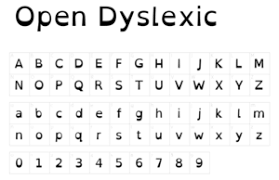
\includegraphics[width=0.92\linewidth]{open_dyslexic.png}
    \caption{Weighted-base OpenDyslexic typeface~\cite{12} integrated into the Synapse typographic engine to mitigate perceived letter inversion.}
    \label{fig:opendyslexic}
\end{figure}

\textit{3) Vision-Based Oculomotor Screening:} Grounded in the magnocellular theory~\cite{13}, infrared eye-tracking benchmarks establish longer fixation durations, gaze instability, and backward regressions as reliable biomarkers of dyslexia~\cite{14}. Translating these clinical markers into real-time consumer browser tools remains difficult without lightweight visual pipelines and behavioral sensor fusion.

\subsection{Architectural Requirements}
Addressing disjointed workflows and passive filtering requires satisfying three structural requirements (summarized in Table~\ref{tab:requirements}):
\begin{enumerate}
    \item \textbf{Non-Intrusive Perceptual Assistance:} Render typographic, spatial, and auditory aids via state-driven overlays without mutating source text.
    \item \textbf{Granular Structural Awareness:} Expose exact viewport geometry for every paragraph, wrapped visual line, sentence, and word token in real time.
    \item \textbf{Dynamic Explainable Adaptation:} Fuse behavioral and lexical cues to predict word-level cognitive load and adapt typography and TTS pacing closed-loop.
\end{enumerate}

\begin{table}[t]
\caption{Mapping Traditional Limitations to Synapse Requirements}
\centering
\begin{tabular}{|p{3.8cm}|p{4.1cm}|}
\hline
\textbf{Traditional Limitation} & \textbf{Synapse Architectural Solution} \\
\hline
Isolated single-modality workflows & Unified React/TypeScript frontend execution \\
\hline
Destructive text formatting & Non-destructive tokenized DOM overlays \\
\hline
Coarse document/sentence granularity & Word \texttt{<span>} + \texttt{getClientRects()} line clustering \\
\hline
Static, passive UI filters & Closed-loop Adaptive Engine + XGBoost/TreeSHAP \\
\hline
Biometric video privacy exposure & 100\% browser-local feature extraction ($<50$\,ms) \\
\hline
\end{tabular}
\label{tab:requirements}
\end{table}

% ==========================
% SECTION III: SYSTEM ARCHITECTURE & ASSISTIVE READER
% ==========================
\section{Unified System Architecture and Assistive Reader}

Synapse executes all perception layers, computer vision inference, behavioral tracking, and ML scoring locally inside the browser to guarantee sub-$50$\,ms responsiveness and strict biometric privacy (Fig.~\ref{fig:architecture}).

\begin{figure*}[t]
    \centering
    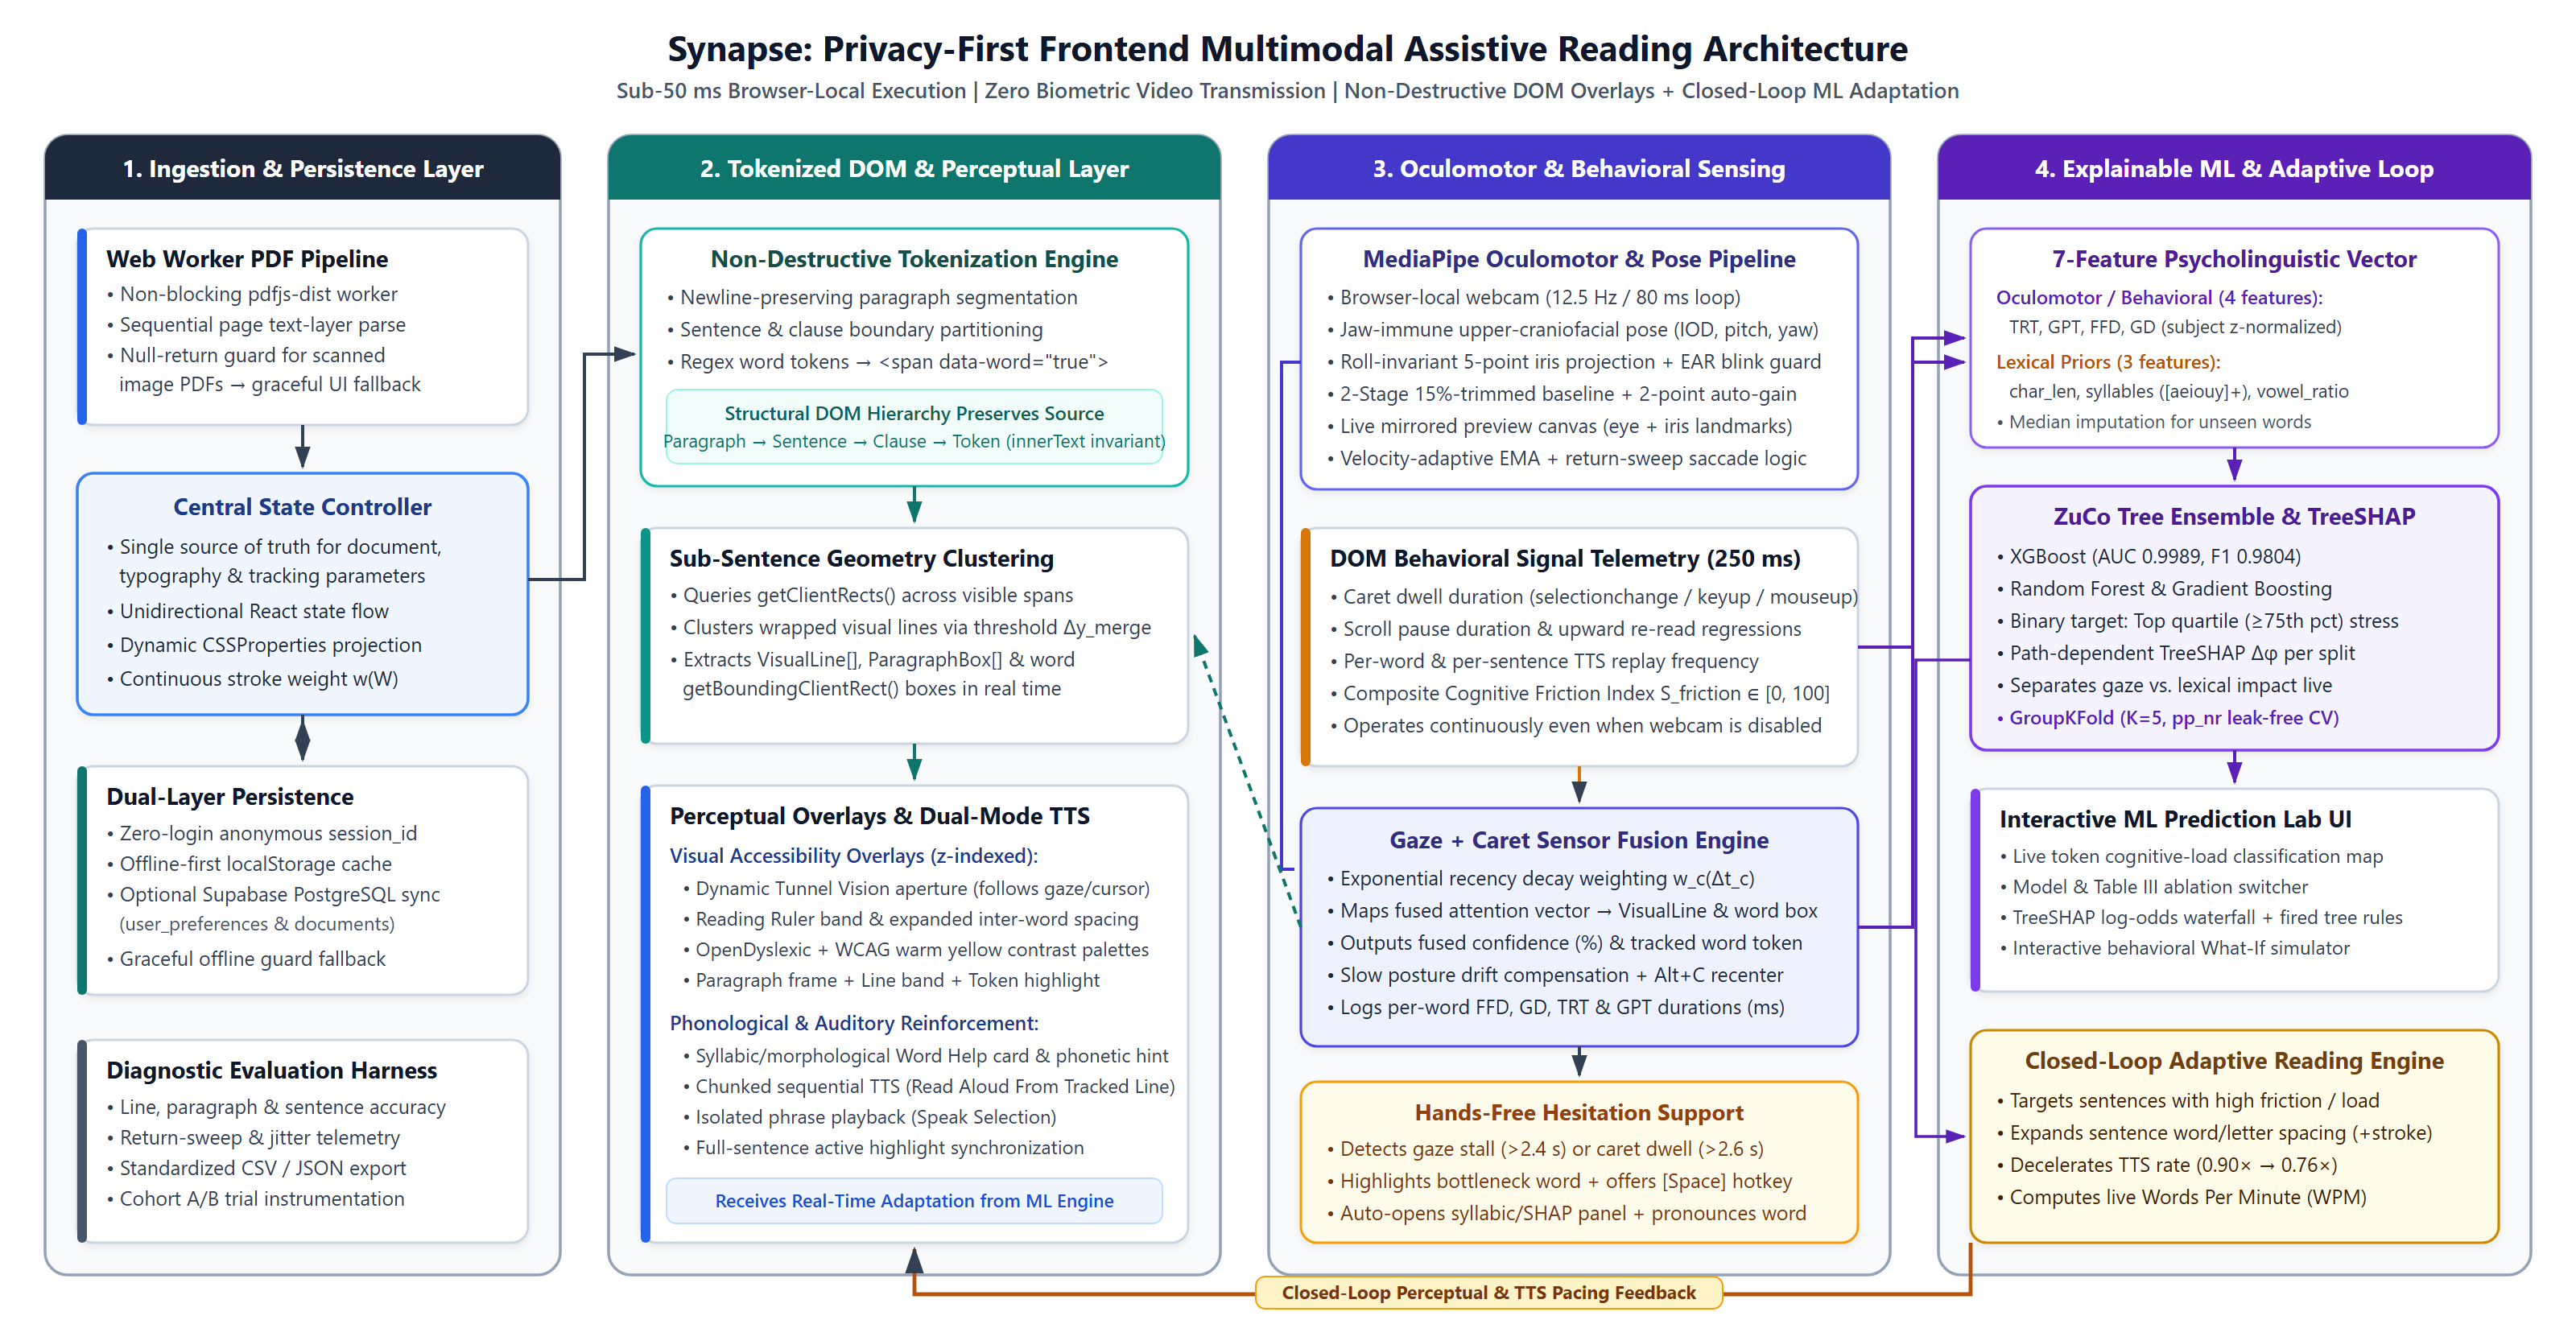
\includegraphics[width=0.98\linewidth]{synapse_system_architecture_300dpi.png}
    \caption{End-to-end multimodal Synapse architecture spanning four browser-local tiers: Web Worker PDF ingestion and dual persistence, hierarchical tokenized DOM overlays, 12.5\,Hz oculomotor + DOM behavioral sensor fusion, and the explainable ZuCo GBDT/TreeSHAP Adaptive Reading Engine.}
    \label{fig:architecture}
\end{figure*}

\subsection{Ingestion, Tokenization, and Visual-Line Clustering}
As a modular serverless web application, the React/TypeScript controller (\texttt{App.tsx}) governs shared reading state, persisting preferences and documents offline-first in \texttt{localStorage} under an anonymous UUID \texttt{session\_id} with optional Supabase PostgreSQL synchronization (\texttt{supabase.ts}), while offloading PDF extraction to a background Web Worker (\texttt{pdfParser.ts}) built on PDF.js~\cite{15}. When an uploaded PDF contains only flattened images without a selectable text layer, the parser returns \texttt{null} and surfaces an accessible fallback prompt rather than stalling the UI. The reading engine (\texttt{TextEditor.tsx}), psycholinguistic ML pipeline (\texttt{zucoFeatureModel.ts}), and interactive explainer (\texttt{MlPredictionLab.tsx}) operate strictly as browser modules without server inference calls.

Rather than a standard \texttt{<textarea>}, text is ingested through a four-level non-destructive HTML pipeline inside a scroll-locked \texttt{contentEditable} container:
\begin{itemize}
    \item \textbf{Paragraph \& Sentence Preservation:} Newline sequences remain verbatim outside span elements so \texttt{innerText} stays invariant to raw source text, while paragraphs and punctuation-delimited sentences receive sequential \texttt{data-paragraph-index} and \texttt{data-sentence-index} attributes.
    \item \textbf{Clause \& Word Tokenization:} Complex sentences ($\ge 16$ words or multi-clause conjunctions) are segmented into toggleable visual clauses, and regular-expression tokenization wraps every word boundary into an addressable \texttt{<span data-word="true">} token.
    \item \textbf{Sub-Sentence Line Clustering:} Because single sentences frequently wrap across multiple rows, querying element-level boxes produces ambiguous multi-line rects. Synapse aggregates \texttt{getClientRects()} fragments across visible spans by vertical midpoint $y_c$ within a font-scaled tolerance:
    \begin{equation}
        \Delta y_{\text{merge}} = \max\!\big(10\text{ px},\; 0.58\, S_{\text{font}}\big),
    \end{equation}
    yielding exact wrapped \texttt{VisualLine} bands and \texttt{ParagraphBox} frames in viewport space.
\end{itemize}

\subsection{Perceptual Overlays and Dual-Mode Auditory Support}
To prevent discrete font steps from stalling between regular ($400$) and bold ($700$) weights, Synapse synthesizes continuous glyph weights across $W \in [300, 900]$ by coupling CSS weight with proportional sub-pixel stroke reinforcement:
\begin{equation}
    w_{\text{stroke}}(W) =
    \begin{cases}
        0\text{ px}, & W \le 400, \\
        \dfrac{W - 400}{500} \times 0.65\text{ px}, & 400 < W \le 900.
    \end{cases}
\end{equation}
Three synchronized perceptual layers overlay the container above the text layer ($z$-indexed safely beneath modal controls): (1) a cursor-following \textbf{Reading Ruler}, (2) \textbf{Dynamic Tunnel Vision}, which positions blurred top and bottom masks around a clear $22\%$ vertical reading aperture tracked to either the active mouse coordinate or live webcam gaze coordinate $Y_{\text{tunnel}}$:
\begin{align}
    H_{\text{top}} &= \text{clamp}(Y_{\text{tunnel}} - 11\%,\; 8\%,\; 76\%), \\
    H_{\text{bot}} &= \text{clamp}(89\% - Y_{\text{tunnel}},\; 8\%,\; 76\%),
\end{align}
and (3) lateral crowding relief (\texttt{word-spacing: 0.45em}). For phonological reinforcement, clicking any token opens a Word Help panel showing prefix/root/suffix morphology, syllabic chunking, phonetic respelling, and rule-based lexical difficulty flags, while the chunked Web Speech TTS engine supports both gaze-anchored sequential reading (highlighting full active sentences cleanly without stalling on unsupported browser word-boundary events) and highlighted-phrase \textbf{Speak Selection} playback.

% ==========================
% SECTION IV: OCULOMOTOR & BEHAVIORAL FUSION
% ==========================
\section{Oculomotor Tracking and Behavioral Sensor Fusion}

To overcome hardware cost and heavyweight Perspective-n-Point latency without remote streaming, Synapse integrates a $12.5$\,Hz ($\Delta t = 80$\,ms) MediaPipe FaceLandmarker pipeline~\cite{16} (WebGL GPU delegate with CPU fallback) with continuous DOM behavioral sensing (Fig.~\ref{fig:calibration_seq}).

\begin{figure*}[t]
    \centering
    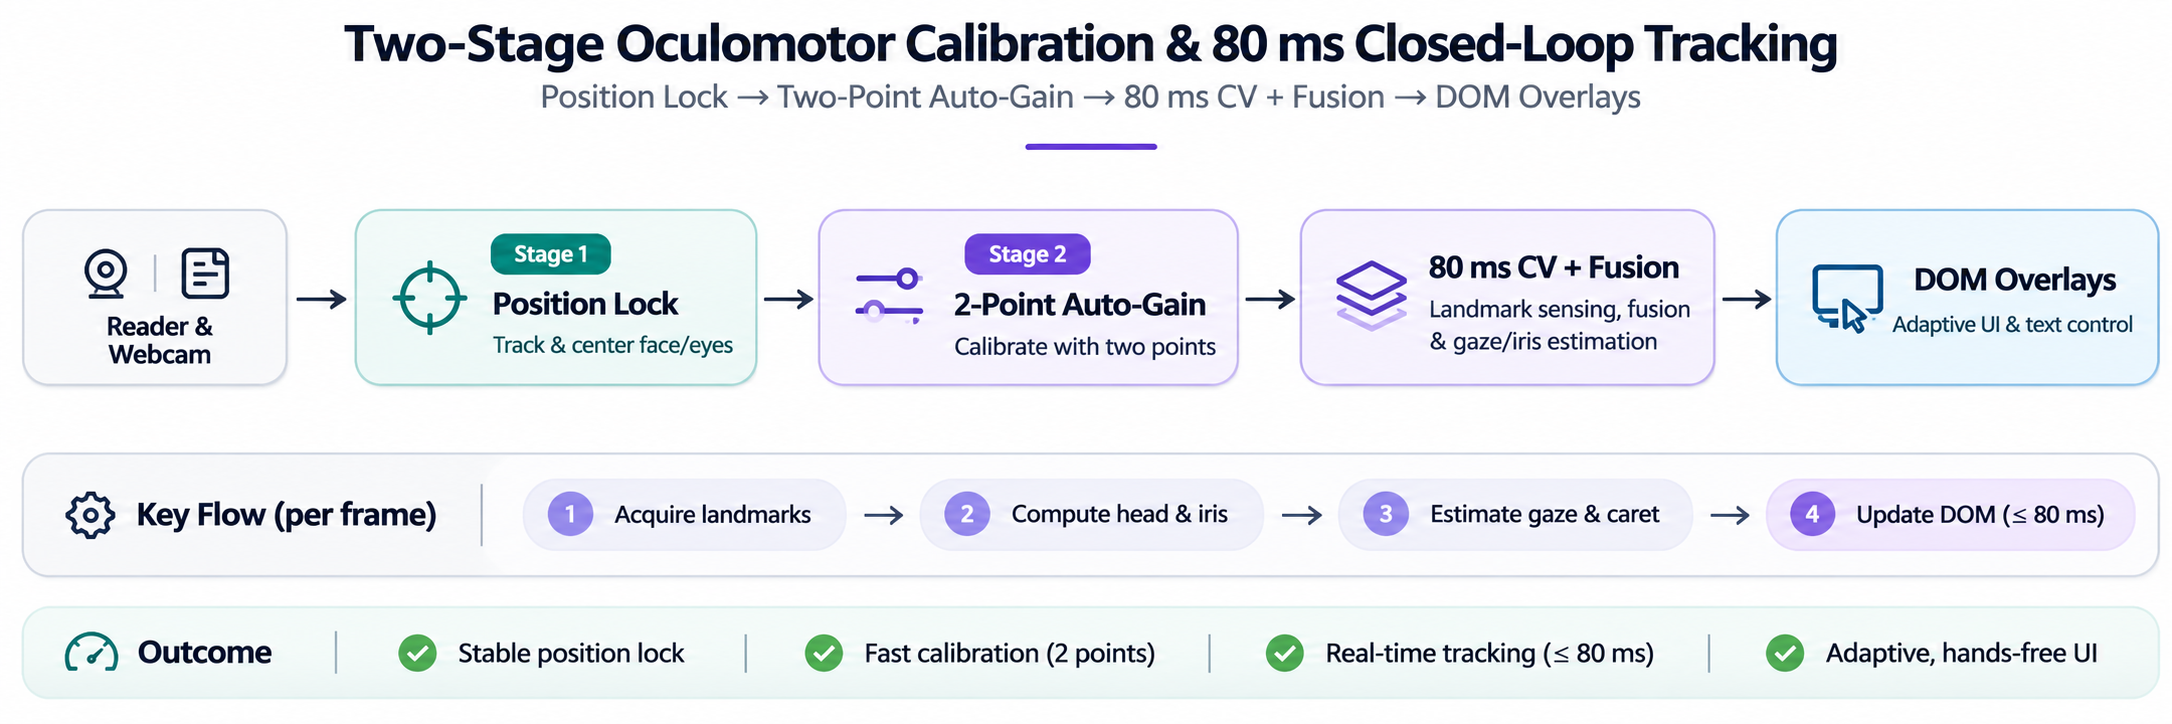
\includegraphics[width=0.96\linewidth]{synapse_calibration_sequence_300dpi.png}
    \caption{Two-stage oculomotor initialization (Step~1 reading-position lock with mirrored eye/iris verification and optional Step~2 two-point auto-gain check) feeding the 80\,ms pose, iris, return-sweep, and DOM behavioral fusion loop.}
    \label{fig:calibration_seq}
\end{figure*}

\subsection{Scale-Invariant Head Pose and Roll-Invariant Iris Projection}
Front-facing camera coordinates $(x_{\text{raw}}, y_{\text{raw}}) \in [0,1]^2$ are mirror-corrected as $x = 1 - x_{\text{raw}}$. To remain invariant to speech and jaw articulation, head pose is derived strictly from rigid upper-craniofacial landmarks: bilateral outer/inner eye corners defining eye centers $\mathbf{c}_L, \mathbf{c}_R$, eye midpoint $\mathbf{m}_{\text{eye}} = (\mathbf{c}_L + \mathbf{c}_R)/2$, and dorsal/tip nasal anchors $\mathbf{n}_{\text{tip}}$. Defining the inter-ocular distance $D_{\text{IOD}} = \|\mathbf{c}_R - \mathbf{c}_L\|_2$ yields scale-normalized pitch and yaw ratios alongside the weighted upper-face anchor $\mathbf{u}_{\text{face}}$:
\begin{equation}
\begin{aligned}
    \mathbf{u}_{\text{face}}
        &= 0.55\,\mathbf{m}_{\text{eye}}
         + 0.45\,\mathbf{n}_{\text{tip}}, \\
    R_{\text{pitch}}
        &= \frac{n_{\text{tip},y} - m_{\text{eye},y}}{D_{\text{IOD}}}, \\
    R_{\text{yaw}}
        &= \frac{n_{\text{tip},x} - m_{\text{eye},x}}{D_{\text{IOD}}}.
\end{aligned}
\end{equation}

For each eye, let $W_{\text{eye}}$ denote canthal width along unit corner axis $\hat{\mathbf{e}} = (e_x, e_y)$, $H_{\text{open}}$ denote vertical eyelid aperture, and $\bar{\mathbf{p}}_{\text{iris}}$ denote the mean centroid of the multi-point iris contour. An Eye Aspect Ratio ($\text{EAR} = H_{\text{open}} / W_{\text{eye}} < 0.14$) blink guard rejects eyelid closure frames and preserves the last valid iris offset. On open eyes, projecting $\mathbf{r} = \bar{\mathbf{p}}_{\text{iris}} - \mathbf{m}_{\text{corner}}$ onto $(\hat{\mathbf{e}}, \hat{\mathbf{e}}_{\perp})$ and blending palpebral-aperture offset $g_{\text{lid}}$ yields roll-invariant normalized iris components $(I_x, I_y) \in [-1,1]^2$:
\begin{equation}
\begin{aligned}
    I_x &= \text{clamp}\!\left(
        3.0\,\frac{\mathbf{r}\cdot\hat{\mathbf{e}}}{W_{\text{eye}}},
        -1,\,1\right), \\
    I_y &= \text{clamp}\!\left(
        3.2\left(
        0.65\,\frac{\mathbf{r}\cdot\hat{\mathbf{e}}_{\perp}}{W_{\text{eye}}}
        + 0.35\,g_{\text{lid}}\right),
        -1,\,1\right).
\end{aligned}
\end{equation}

\subsection{Two-Stage Calibration, Return Sweeps, and Posture Drift}
During \textbf{Step~1 (Reading Position Initialization)}, a mirrored landmark canvas verifies eye/iris lock while the reader selects or fixates on a starting line $L_{\text{target}}$. Over $2.1$\,s ($N \ge 12$ samples), $15\%$-trimmed means establish personal head ($\mathbf{H}_0$) and iris ($\mathbf{I}_0$) baselines plus neutral line height $Y_0 \in [0.15, 0.75]$, unlocking \textbf{Step~2 (Fine-Tuning \& Two-Point Auto-Gain)}. During the optional 2-point top/bottom gaze check over screen span $\Delta Y_{\text{screen}} = Y_{\text{bot}} - Y_{\text{top}}$, observed vertical head excursion $\Delta H_{\text{obs},y}$ and iris excursion $\Delta I_{\text{obs},y}$ automatically calibrate sensitivity gains via head share:
\begin{equation}
    \rho_{\text{head}} =
    \text{clamp}\!\left(
    \frac{\Delta H_{\text{obs},y}}
         {\Delta H_{\text{obs},y}+0.35\,\Delta I_{\text{obs},y}},
    0.38,\,0.72\right).
\end{equation}
The calibrated gains are:
\begin{equation}
\begin{aligned}
    K_{\text{head}}^{\star}
        &= \text{clamp}\!\left(
        \frac{\Delta Y_{\text{screen}}\,\rho_{\text{head}}}
             {\Delta H_{\text{obs},y}},
        0.90,\,2.85\right), \\
    K_{\text{iris}}^{\star}
        &= \text{clamp}\!\left(
        \frac{\Delta Y_{\text{screen}}(1-\rho_{\text{head}})}
             {1.45\,\Delta I_{\text{obs},y}},
        0.08,\,0.62\right).
\end{aligned}
\end{equation}

In active mode, distance-scaled pose deviations ($s = D_{\text{IOD},0}/D_{\text{IOD}}$) and iris deltas combine into gaze point $\mathbf{p}_{\text{gaze}} = (x_{\text{gaze}}, y_{\text{gaze}})$, filtered by a velocity-adaptive Exponential Moving Average ($\alpha_y \in [0.22, 0.62]$; $\alpha_x = 0.76$ on leftward sweeps, else $[0.25, 0.65]$). To capture end-of-line transitions instantaneously without waiting for multi-hit debounce, a \textbf{Return-Sweep Saccade Detector} advances directly from $L_k$ to $L_{k+1}$ whenever horizontal progress drops sharply from the right half ($P_{\max,x} \ge 0.56$) back leftward ($P_{\max,x} - P_x \ge 0.26$, $P_x \le 0.44$) within $L_{k+1}$'s vertical neighborhood, applying an exponentially decaying offset $\Delta y_{\text{sweep}}$ to prevent line bounce-back. Slow baseline drift during steady reading is absorbed continuously ($\eta_x = 0.004, \eta_y = 0.0028$), and shortcut \texttt{Alt+C} provides instant single-frame recentering.

\subsection{DOM Behavioral Signals and Gaze + Caret Fusion}
Complementing webcam tracking---and functioning autonomously when no camera is active---a $250$\,ms DOM telemetry loop records caret dwell time $\tau_{\text{caret}}$, scroll pauses $N_{\text{pause}}$ ($\ge 2.2$\,s), upward re-read regressions $N_{\text{reg}}$ ($\Delta S_y < -22$\,px), gaze hesitation stalls $N_{\text{gaze}}$ ($\ge 2.4$\,s), caret friction stalls $N_{\text{caret}}$ ($\ge 2.6$\,s), and cumulative sentence/word TTS replays $N_{\text{replay}}$, synthesizing a bounded composite friction index:
\begin{equation}
\begin{aligned}
    S_{\text{friction}} = \text{clamp}\Big(&
        \min\!\big(28,\,\lfloor\tau_{\text{caret}}/350\rfloor\big) \\
        &+ 12(N_{\text{caret}} + N_{\text{gaze}}) \\
        &+ \min\!\big(24,\,9N_{\text{reg}}+3N_{\text{pause}}\big) \\
        &+ \min\!\big(36,\,12N_{\text{replay}}\big),
        \;0,\,100\Big).
\end{aligned}
\end{equation}
When a DOM caret anchor $\mathbf{p}_{\text{caret}}$ has moved recently ($\Delta t_c < 14$\,s) near the active gaze neighborhood, exponential recency fusion blends both signals:
\begin{equation}
\begin{aligned}
    w_c(\Delta t_c)
        = \text{clamp}\!\Bigg(&0.10 + 0.32\,
        \exp\!\left(-\frac{\Delta t_c}{6000\text{ ms}}\right),\\
        &0.10,\,0.42\Bigg).
\end{aligned}
\end{equation}
updating the active attention vector as $\mathbf{p}_{\text{fused}} = (1 - w_c)\,\mathbf{p}_{\text{gaze}} + w_c\,\mathbf{p}_{\text{caret}}$ and snapping to the nearest \texttt{VisualLine} and tokenized word bounding box. Gaze stalls $>2.4$\,s or caret stalls $>2.6$\,s on tricky words highlight the token and offer a hands-free \texttt{Space} shortcut to open its syllabic and SHAP panel.

% ==========================
% SECTION V: EXPERIMENTAL RESULTS & ADAPTIVE ENGINE
% ==========================
\section{Experimental Results: ZuCo Cognitive Difficulty Prediction and Closed-Loop Adaptation}

\subsection{Dataset, Subject Normalization, and Feature Engineering}
Model evaluation utilized the Zurich Cognitive Language Processing Corpus (ZuCo)~\cite{17}, merging L1 and L2 natural reading tasks. Raw eye-tracking metrics were first $z$-score normalized per subject ($z_{i,j} = (x_{i,j} - \mu_{p,j})/\sigma_{p,j}$) to remove baseline speed bias. Aggregating median normalized gaze metrics produced a word-level composite stress score; tokens in the top quartile ($\ge 0.75$ quantile) formed the difficult class (\texttt{is\_difficult} $= 1$), with the remaining tokens forming the baseline class ($0$). Seven features were extracted per word token:
\begin{itemize}
    \item \textbf{Lexical Features (3):} Character length (\texttt{char\_len}), vowel-group syllable count (\texttt{[aeiouy]+}), and \texttt{vowel\_ratio}.
    \item \textbf{Gaze/Behavioral Features (4):} Total reading time (\texttt{word\_total\_reading\_time}), go-past duration (\texttt{word\_go\_past\_time}), first fixation duration (\texttt{word\_first\_fixation\_duration}), and first-pass gaze duration (\texttt{word\_gaze\_duration}), with continuous median imputation for unfixated tokens.
\end{itemize}

\subsection{Ensemble Models, 5-Fold GroupKFold Ablation, and Performance}
Experiments executed on an NVIDIA Tesla P100 GPU evaluated Random Forest ($500$ trees, balanced class weights), Gradient Boosting ($300$ trees, $\text{lr}=0.05$), and XGBoost~\cite{18} ($800$ trees, $\text{max\_depth}=6$, $\text{lr}=0.03$, \texttt{tree\_method="hist"}, subsample/colsample $=0.8$). To guarantee zero participant data leakage, evaluation used $K=5$ \texttt{GroupKFold} cross-validation grouped strictly by subject ID (\texttt{pp\_nr}) across three feature configurations: Lexical-Only, Gaze-Only, and Combined (Table~\ref{tab:ablation_results}).

\begin{table}[t]
\caption{5-Fold GroupKFold Cross-Validation Ablation Results on ZuCo (Mean $\pm$ SD)}
\centering
\small
\setlength{\tabcolsep}{2pt}
\begin{tabular}{|p{1.35cm}|p{1.45cm}|c|c|}
\hline
\textbf{Feature Set} & \textbf{Model} & \textbf{Mean ROC-AUC} & \textbf{Mean F1} \\
\hline
\multirow{3}{1.35cm}{\centering Lexical Only}
 & Random Forest & $0.6430 \pm 0.0106$ & $0.4254 \pm 0.0747$ \\
 & Gradient Boosting & $0.6433 \pm 0.0109$ & $0.0751 \pm 0.0250$ \\
 & XGBoost & $0.6432 \pm 0.0106$ & $0.0725 \pm 0.0237$ \\
\hline
\multirow{3}{1.35cm}{\centering Gaze Only}
 & Random Forest & $0.9980 \pm 0.0002$ & $0.9796 \pm 0.0040$ \\
 & Gradient Boosting & $0.9984 \pm 0.0004$ & $0.9775 \pm 0.0053$ \\
 & XGBoost & $0.9989 \pm 0.0002$ & $0.9806 \pm 0.0034$ \\
\hline
\multirow{3}{1.35cm}{\centering Combined}
 & Random Forest & $0.9986 \pm 0.0003$ & $0.9798 \pm 0.0039$ \\
 & Gradient Boosting & $0.9984 \pm 0.0004$ & $0.9775 \pm 0.0054$ \\
 & \textbf{XGBoost (Best)} & $\mathbf{0.9989 \pm 0.0002}$ & $\mathbf{0.9804 \pm 0.0039}$ \\
\hline
\end{tabular}
\label{tab:ablation_results}
\end{table}

Lexical features alone achieved at most Mean AUC $0.6433$, demonstrating that surface orthography cannot predict individual reader bottlenecks. Adding oculomotor features raised Mean AUC to $0.9989$ ($\text{F1}=0.9804$) under Combined XGBoost, confirming that cognitive reading difficulty is fundamentally an interaction-driven behavioral phenomenon.

\subsection{TreeSHAP Explainability and In-Browser ML Inference Lab}
To maintain clinical transparency, SHapley Additive exPlanations (SHAP)~\cite{19} were extracted via \texttt{TreeExplainer}, decomposing predictions additively across tree paths:
\begin{equation}
\begin{aligned}
    f(\mathbf{x}) &= \phi_0 + \sum_{j=1}^{7}\phi_j(\mathbf{x}), \\
    \Delta\phi_{j_m}^{(t)}
        &= w_t\!\left(
        \mathbb{E}[f_t \mid v_{m+1}]
        - \mathbb{E}[f_t \mid v_m]\right).
\end{aligned}
\end{equation}
As illustrated in Fig.~\ref{fig:shap_analysis}, behavioral gaze durations---specifically \texttt{word\_total\_reading\_time} and \texttt{word\_go\_past\_time}---account for the overwhelming majority of total absolute SHAP attribution, pushing high-duration tokens decisively toward Class~1 while lexical priors cluster near zero to stabilize cold-start edge cases.

\begin{figure}[t]
    \centering
    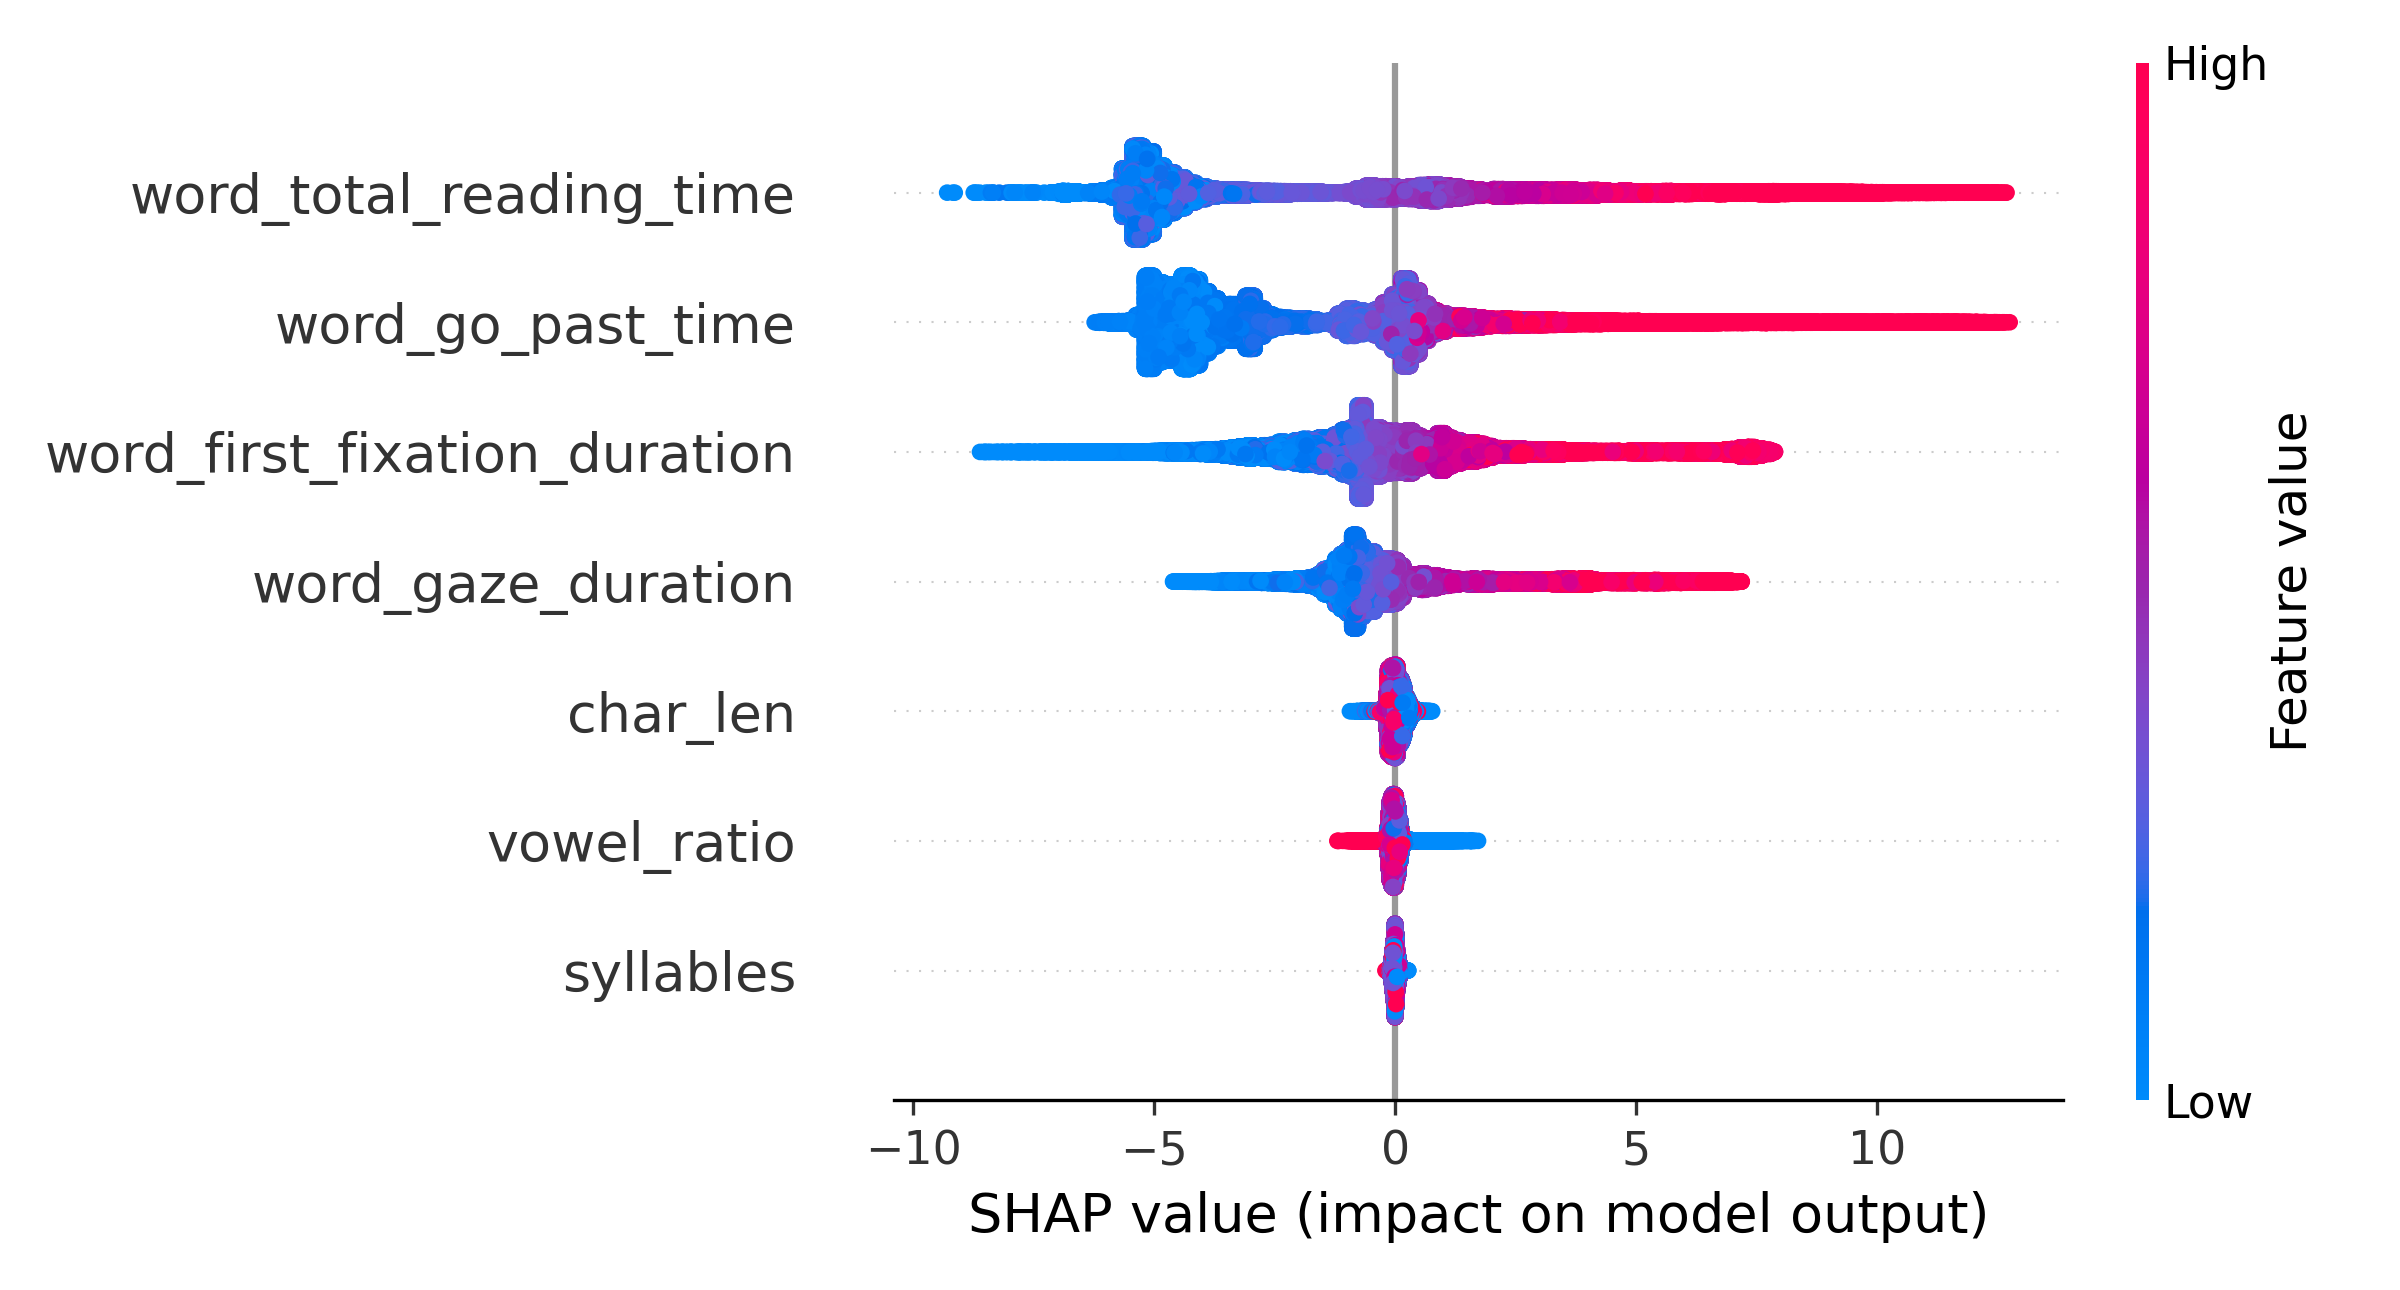
\includegraphics[width=0.98\linewidth]{shap_summary.png}
    \caption{TreeSHAP summary plot on the Combined XGBoost model. Temporal gaze features (\texttt{word\_total\_reading\_time}, \texttt{word\_go\_past\_time}) dominate model attribution over static lexical features.}
    \label{fig:shap_analysis}
\end{figure}

Within the Synapse web client, a calibrated decision-tree ensemble and path-dependent TreeSHAP engine (\texttt{zucoFeatureModel.ts}) runs live inference over DOM/webcam word observations and powers an interactive \textbf{ML Prediction Lab} (\texttt{MlPredictionLab.tsx}). Users and researchers can toggle classifiers and Table~\ref{tab:ablation_results} ablation subsets, inspect token-level probability heatmaps, view live SHAP waterfalls and fired tree split rules, or simulate reading stalls interactively.

\subsection{Closed-Loop Adaptive Reading Engine and Diagnostic Harness}
Completing the system feedback loop, the opt-in \textbf{Adaptive Reading Engine} dynamically modifies rendering solely on sentences flagged by repeated TTS replays ($c_s \ge 2$), dwell stalls, or extended observed word durations ($\text{TRT} \ge 900$\,ms), applying wider inter-word spacing ($0.38$\,em), stroke weight reinforcement, and automated TTS rate deceleration from $0.90\times$ to $0.76\times$ while tracking live Words Per Minute (WPM). In addition, Synapse includes a standalone client-side \textbf{Diagnostic Evaluation Harness} instrumented to record face/iris lock availability, visual-line and paragraph exact/adjacent match rates, return-sweep triggers, and switching jitter for standardized export in CSV and JSON during controlled user studies.

% ==========================
% SECTION VI: DISCUSSION, LIMITATIONS, AND FUTURE WORK
% ==========================
\section{Discussion, Limitations, and Future Work}

\subsection{Privacy and Linguistic Generalization}
Processing raw webcam imagery, caret positions, and scroll dynamics exclusively inside browser memory ensures strict educational data privacy without remote biometric streaming; optional synchronization handles only user preferences and saved documents. Synapse's modular separation between orthographic heuristics (\texttt{pronunciation.ts}, \texttt{wordDifficulty.ts}) and oculomotor/DOM sensing further supports adaptation across shallow and deep orthographies without altering the core tracking engine.

\subsection{Limitations: Bridging the Webcam Tracking Gap}
While our earlier CNN prototypes using OpenFace~\cite{20}, MTCNN~\cite{21}, and CLNF~\cite{22} suffered prohibitive Perspective-n-Point latency in serverless browsers, Synapse bridges this architectural gap through browser-native MediaPipe FaceLandmarker~\cite{16}, two-point auto-gain calibration, return-sweep heuristics, and DOM gaze + caret sensor fusion. Nevertheless, an ecological accuracy gap persists between clinical infrared hardware used in ZuCo ($1000$\,Hz) and noisy consumer RGB webcams ($30$\,Hz sampling, $12.5$\,Hz inference) affected by eyeglasses glare, ambient lighting variance, and head motion. Accordingly, while offline predictive accuracy on ZuCo reaches AUC $0.9989$ and the diagnostic evaluation harness is fully instrumented, \textbf{longitudinal clinical A/B user trials with dyslexic cohorts}---evaluating live WPM, reading accuracy, tracking precision, and comprehension retention against non-adaptive interfaces---remain the essential next validation phase.

% ==========================
% SECTION VII: CONCLUSION
% ==========================
\section{Conclusion}

Existing dyslexia technologies isolate typography, speech assistance, and oculomotor screening into fragmented tools. Synapse unifies these modalities within a privacy-first, frontend-resident platform built atop a non-destructive tokenized \texttt{contentEditable} DOM. By combining continuous perceptual and phonological aids, calibrated browser-local head+iris tracking with return-sweep detection, DOM behavioral friction sensing, and an explainable ZuCo XGBoost/TreeSHAP Adaptive Reading Engine (AUC $0.9989 \pm 0.0002$), Synapse establishes an end-to-end foundation for proactive, personalized reading support that observes and adapts to cognitive difficulty in real time.

\section*{Data and Code Availability}
The Zurich Cognitive Language Processing Corpus (ZuCo)~\cite{17} used for model training and 5-fold cross-validation is publicly available. All Synapse frontend modules, tokenization utilities, Attention Tracking Diagnostic Harness, and trained ZuCo ML/SHAP artifacts will be released in an anonymized public repository upon publication.

% ==========================
% REFERENCES [1] - [22]
% ==========================
\begin{thebibliography}{00}

\bibitem{1}
D. L. Lefly and B. F. Pennington,
``Reliability and validity of the Adult Reading History Questionnaire,''
\textit{Journal of Learning Disabilities}, vol. 33, no. 3, pp. 286--296, 2000.

\bibitem{2}
A. J. Fawcett and R. I. Nicolson,
\textit{Dyslexia Screening Test (DST)},
London, U.K.: Harcourt Assessment, 1996.

\bibitem{3}
A. Khalid, M. Zaffar, and M. Ramzan,
``Assistive technologies for dyslexia: A review,''
\textit{IEEE Access}, vol. 8, pp. 64589--64609, 2020.

\bibitem{4}
M. J. Snowling,
\textit{Dyslexia},
Oxford, U.K.: Blackwell Publishing, 2000.

\bibitem{5}
E. L. F. da Silva, R. S. Guti\'errez, and A. P. C. da Silva,
``Using acoustic features to identify speech difficulties associated with dyslexia,''
\textit{International Journal of Speech Technology}, vol. 22, pp. 601--612, 2019.

\bibitem{6}
E. L. F. da Silva \textit{et al.},
``Automatic detection of reading difficulties using speech alignment patterns,''
in \textit{Proc. IEEE Int. Conf. Acoustics, Speech and Signal Processing (ICASSP)}, 2021, pp. 7428--7432.

\bibitem{7}
S. Cox and S. Dasmahapatra,
``High-level approaches to confidence estimation in speech recognition,''
\textit{IEEE Transactions on Speech and Audio Processing}, vol. 10, no. 7, pp. 460--471, 2002.

\bibitem{8}
A. D. Baddeley and G. Hitch,
``Working memory,''
\textit{Psychology of Learning and Motivation}, vol. 8, pp. 47--89, 1974.

\bibitem{9}
J. Sweller,
``Cognitive load during problem solving: Effects on learning,''
\textit{Cognitive Science}, vol. 12, no. 2, pp. 257--285, 1988.

\bibitem{10}
H. Irlen,
\textit{Reading by the Colors: Overcoming Dyslexia and Other Reading Disabilities Through the Irlen Method},
New York, NY, USA: Avery Publishing, 2005.

\bibitem{11}
S. N. Abdul Wahid,
``Evaluation of dyslexia-friendly fonts for improved readability,''
\textit{International Journal of Education and Literacy}, 2017.

\bibitem{12}
A. Gonzalez,
``OpenDyslexic: A typeface for dyslexia,''
OpenDyslexic, 2011. [Online]. Available: \url{https://opendyslexic.org}

\bibitem{13}
J. Stein,
``The magnocellular theory of developmental dyslexia,''
\textit{Dyslexia}, vol. 7, no. 1, pp. 12--36, 2001.

\bibitem{14}
M. N. Benfatto \textit{et al.},
``Screening for dyslexia using eye tracking during reading,''
\textit{Journal of Learning Disabilities}, vol. 49, no. 2, pp. 196--208, 2016.

\bibitem{15}
Mozilla Foundation,
``PDF.js: A general-purpose, web standards-based platform for parsing and rendering PDFs,''
2024. [Online]. Available: \url{https://mozilla.github.io/pdf.js/}

\bibitem{16}
Y. Kartynnik \textit{et al.},
``Real-time facial surface geometry from monocular video on mobile GPUs,''
in \textit{CVPR Workshop on Computer Vision for Augmented and Virtual Reality}, 2019 (MediaPipe FaceMesh / FaceLandmarker).

\bibitem{17}
N. Hollenstein \textit{et al.},
``ZuCo, a simultaneous EEG and eye-tracking resource for sentence reading,''
\textit{Scientific Data}, vol. 5, no. 1, pp. 1--13, 2018.

\bibitem{18}
T. Chen and C. Guestrin,
``XGBoost: A scalable tree boosting system,''
in \textit{Proc. 22nd ACM SIGKDD Int. Conf. Knowledge Discovery and Data Mining}, 2016, pp. 785--794.

\bibitem{19}
S. M. Lundberg and S.-I. Lee,
``A unified approach to interpreting model predictions,''
in \textit{Advances in Neural Information Processing Systems (NeurIPS)}, vol. 30, 2017.

\bibitem{20}
T. Baltru\v{s}aitis, P. Robinson, and L.-P. Morency,
``OpenFace: An open source facial behavior analysis toolkit,''
in \textit{Proc. IEEE Winter Conf. Applications of Computer Vision (WACV)}, 2016, pp. 1--10.

\bibitem{21}
K. Zhang, Z. Zhang, Z. Li, and Y. Qiao,
``Joint face detection and alignment using multitask cascaded convolutional networks,''
\textit{IEEE Signal Processing Letters}, vol. 23, no. 10, pp. 1499--1503, 2016.

\bibitem{22}
T. Baltru\v{s}aitis, P. Robinson, and L.-P. Morency,
``Constrained local neural fields for robust facial landmark detection in the wild,''
in \textit{Proc. IEEE Int. Conf. Computer Vision Workshops (ICCVW)}, 2013, pp. 354--361.

\end{thebibliography}

\end{document}
